\documentclass[12pt]{article}

% ---------- Packages ----------
\usepackage[a4paper,margin=1in]{geometry}
\usepackage{amsmath,amssymb,amsthm,mathtools}
\usepackage{bm}
% \usepackage{physics} % removed to avoid macro conflicts
\usepackage{siunitx}
\usepackage{booktabs}
\usepackage{array}
\usepackage{longtable}
\usepackage{enumitem}
\usepackage{hyperref}
\usepackage[nameinlink]{cleveref}
\usepackage[most]{tcolorbox}
\usepackage{xcolor}
\usepackage{microtype}
\usepackage{tikz}
\usetikzlibrary{arrows.meta,positioning,calc,fit,decorations.pathmorphing}
\usepackage{subcaption}
\usepackage{listings}
\lstdefinestyle{codeblock}{%
  basicstyle=\ttfamily\small,
  frame=single,
  frameround=ffff,
  breaklines=true,
  columns=fullflexible,
  keepspaces=true
}
\hypersetup{colorlinks=true,linkcolor=blue,citecolor=blue,urlcolor=blue}

% siunitx setup (v3-safe defaults)
\sisetup{per-mode=symbol, separate-uncertainty=true}

% Cleveref naming (short, journal-style)
\crefname{theorem}{Thm.}{Thms.}
\Crefname{theorem}{Theorem}{Theorems}
\crefname{proposition}{Prop.}{Props.}
\Crefname{proposition}{Proposition}{Propositions}
\crefname{lemma}{Lemma}{Lemmas}
\crefname{corollary}{Cor.}{Cors.}
\Crefname{corollary}{Corollary}{Corollaries}
\crefname{equation}{Eq.}{Eqs.}
\Crefname{equation}{Equation}{Equations}
\crefname{figure}{Fig.}{Figs.}
\Crefname{figure}{Figure}{Figures}

% ---------- Theorem styles ----------
\newtheorem{theorem}{Theorem}[section]
\newtheorem{proposition}[theorem]{Proposition}
\newtheorem{lemma}[theorem]{Lemma}
\newtheorem{corollary}[theorem]{Corollary}
\theoremstyle{definition}
\newtheorem{definition}[theorem]{Definition}
\newtheorem{assumption}[theorem]{Assumption}
\newtheorem{remark}[theorem]{Remark}
\newtheorem{example}[theorem]{Example}

% ---------- Boxed environments ----------
\tcbset{%
  colback=white,
  colframe=black,
  boxsep=4pt,
  arc=1pt,
  outer arc=1pt,
  left=6pt,right=6pt,top=6pt,bottom=6pt
}
% \newtcolorbox{boxed}[1][]{enhanced,breakable,title=#1}
\newtcolorbox{summarybox}{enhanced,breakable,colframe=black!60!white,colback=black!1!white}
\newtcolorbox{algobox}{enhanced,breakable,colframe=black,colback=black!1!white,title=Algorithm}

% ---------- Macros ----------
\newcommand{\R}{\mathbb{R}}
\newcommand{\C}{\mathbb{C}}
\newcommand{\Z}{\mathbb{Z}}
\newcommand{\T}{\mathbb{T}}
\newcommand{\E}{\mathbb{E}}
\newcommand{\Var}{\mathrm{Var}}
\newcommand{\Cov}{\mathrm{Cov}}
\newcommand{\sgn}{\mathrm{sgn}}
\newcommand{\Id}{\mathrm{Id}}
\newcommand{\tr}{\mathrm{tr}}
\newcommand{\diag}{\mathrm{diag}}
\newcommand{\defeq}{\coloneqq}
% Paired delimiters (mathtools) replacing manual \abs,\norm,\ip definitions
\DeclarePairedDelimiter{\ip}{\langle}{\rangle}
\DeclarePairedDelimiter{\norm}{\lVert}{\rVert}
\DeclarePairedDelimiter{\abs}{\lvert}{\rvert}
\newcommand{\bigO}{\mathcal{O}}
\newcommand{\Hinf}{\mathcal{H}^\infty}
\newcommand{\Htwo}{\mathcal{H}^2}
\newcommand{\zunit}{\{z\in\C: \abs{z}=1\}}
\newcommand{\angles}[1]{\langle #1\rangle}

% ---------- Title ----------
\title{\bf Temporal Genesis: A Self-Contained Master Document\\
\large A simple, intuitive, and mathematically consistent story}
\author{Compiled Synthesis}
\date{\today}

\begin{document}
\maketitle
\tableofcontents

\begin{abstract}
We synthesize a complete, self-contained narrative---\emph{temporal genesis}---that turns a timeless description into operational dynamics using signal processing, matrix identities, and covariant limits. The spine is: (i) an exact two-step recursion on decimated residue tracks (Cayley--Hamilton), (ii) a compact \emph{wheel} dictionary that equates this recursion to a dominant conjugate pole pair, (iii) a \emph{Mirror--Outer Spectral Content} (MOSC) operator that preserves spectral magnitude while stripping all-pass phase, (iv) an operational dephasing index tied to phase-increment noise, (v) a binary \emph{APBC} flip mechanism for measurement and Born statistics, and (vi) an emergent Lorentz sector with a dynamic envelope whose strength depends on the decoherence field, producing an effective metric. All non-standard terms are defined; key claims are proved or sketched. We include diagnostics, a practitioner pipeline, and appendices with derivations and ray-tracing pseudo-code.
\end{abstract}

\section{Roadmap and executive summary}
\begin{summarybox}
\textbf{From conditioning to a two-step law.} Condition a timeless global state on a clock sector. On decimated residue tracks one obtains an \emph{exact} recursion
\begin{equation}
y_{k+2}-V_\ell\,y_{k+1}+Q_\ell\,y_k=0,\quad (V_\ell,Q_\ell)=(\tr M^\ell,\ (\det M)^\ell),
\label{eq:two-step}
\end{equation}
where $M\in\C^{2\times2}$ is a reduced transfer and $\ell\in\Z_{>0}$ a stride.

\textbf{Wheel (dominant pair).} If $r_\pm=\rho e^{\pm i\theta}$ dominates, then
\begin{equation}
(V,Q)=(2\rho\cos\theta,\ \rho^2),\qquad V_\ell=2\rho^\ell\cos(\ell\theta),\ \ Q_\ell=\rho^{2\ell}.
\label{eq:wheel}
\end{equation}

\textbf{MOSC.} Factor $H=O\cdot I$ (outer $\times$ inner/all-pass) and define $\mathcal{S}[H]\defeq H/I$. Then $\abs{\mathcal{S}[H]}=\abs{H}$ on the unit circle; $\mathcal{S}[H]$ is outer (minimum-phase).

\textbf{Coherence \& dephasing.} Demodulate by $r_+$, form wrapped phase increments $\delta_t$. Coherence decays as
\begin{equation}
\abs{\mathcal{C}(t)}\approx \rho^{\,t}\,e^{-Dt},\quad D=\tfrac12 S_\delta(0).
\label{eq:coherence}
\end{equation}

\textbf{Measurement as APBC flips.} Micro-absorbers flip PBC$\to$APBC with hazard $\lambda\propto\abs{\phi}^2$, marking $V\mapsto -V$ and yielding Born statistics via first-arrival. Which-path visibility $\sim e^{-D_{\rm proper}T_{\rm proper}}$.

\textbf{Lorentz sector and dynamic envelope.} The coherent AR(2) sector has a KG limit. A dynamic envelope $s=s_0+\alpha S_\delta$ renormalizes the local wave speed, defining an effective metric $g$ and closing a self-consistent gravity--locality loop.

\textbf{Gravity map.} $\Phi\propto S_\delta(0)$ gives quasi-static screened Poisson; dynamics follow a telegraph/KG closure with speed $\le v_{\max}$ and screening length tied to $s$.
\end{summarybox}

\section{Preliminaries, notation, and standard background}
\subsection*{Global conventions and harmonization}
\begin{summarybox}
\textbf{Metric/sign.} We use the ``mostly minus'' convention $\eta=\mathrm{diag}(1,-1,-1,-1)$ and the d'Alembertian
\(
\Box\defeq \frac{1}{c^2}\partial_t^2-\nabla^2.
\)

\textbf{Mass/frequency.} The Klein--Gordon mass parameter is $m$; earlier frequency notation relates via $m\equiv \omega_0/c$.

\textbf{Proper-time dephasing.} Define $\mathcal S(x)$ per proper time; $D_{\rm proper}=\tfrac12\mathcal S$.
Under a constant boost with dilation factor $\gamma$, the coordinate-time dephasing rate scales as
$D=\gamma D_{\rm proper}$ (the zero-frequency PSD scales covariantly under time stretching), so
$\abs{\mathcal C(t)}\sim e^{-Dt}$ becomes $e^{-\gamma D_{\rm proper} t}$.

\textbf{Effective metric.} A dynamic envelope yields $c_{\rm eff}^2=c^2-2\sigma$ with $\sigma=s/\tau^2$, producing an effective metric $g^{00}=1$, $g^{ij}=-(c_{\rm eff}^2/c^2)\delta^{ij}$ in which the principal symbol is Lorentzian.
\end{summarybox}

\subsection{Signals, $z$-transform, and LTI systems}
We consider complex, discrete-time signals $x:\Z\to\C$, with $z$-transform $X(z)=\sum_{t\in\Z} x_t z^{-t}$. A causal, stable LTI system has transfer $H(z)$ analytic on $\abs{z}\ge1$. For AR($p$),
\begin{equation}
H(z)=\frac{\sigma}{A(z)}=\frac{\sigma}{1-a_1 z^{-1}-\dots-a_p z^{-p}},
\end{equation}
with poles $p_j$ inside the unit disk for stability.

\subsection{Hardy spaces, inner/outer, and all-pass}
Let $\Htwo$ be analytic functions on the unit disk with square-integrable boundary values; $\Hinf$ are bounded functions. An \emph{inner} $I\in\Hinf$ has $\abs{I(e^{i\omega})}=1$ a.e.; an \emph{outer} $O\in\Htwo$ has logarithmic magnitude averaging property. Every nonzero $H\in\Htwo$ factors uniquely (up to a unimodular constant) as $H=O\cdot I$.

\subsection{Blaschke products (all-pass building blocks)}
For $\abs{p}<1$,
\(
B_p(z)=\frac{1-\bar p z^{-1}}{1-p z^{-1}}
\)
is inner; finite products build the inner factor.

\subsection{Cayley--Hamilton for $2\times2$ matrices}
Every $M\in\C^{2\times2}$ satisfies $M^2-(\tr M)M+(\det M)\Id=0$. The same holds for $M^\ell$.

\subsection{Page--Wootters conditioning and residue tracks}
We adopt a Page--Wootters view in which a timeless state is conditioned on a clock sector, yielding an ordered stream. For stride $\ell$, residue tracks are decimated sequences $y_k^{(r)}=x_{r+k\ell}$. A \emph{reduced transfer} $M$ acts on a two-dimensional sufficient state across decimated steps.

\section{Exact two-step law from Cayley--Hamilton}
Applying Cayley--Hamilton to $M^\ell$ yields the exact recursion \eqref{eq:two-step} for any linear readout on residue tracks.

\section{The wheel: AR(2) dictionary for a dominant conjugate pair}
If a conjugate pair $r_\pm=\rho e^{\pm i\theta}$ dominates, then \eqref{eq:wheel} holds. The stride-$\ell$ versions follow as shown.

\section{Mirror--Outer Spectral Content (MOSC)}
\begin{definition}[MOSC]
For stable rational $H$ with inner $I$ (finite Blaschke product) and outer $O$, define
\begin{equation}
\mathcal{S}[H]\defeq \frac{H}{I}.
\label{eq:mosc-def}
\end{equation}
\end{definition}
\begin{proposition}[Magnitude preservation]\label{prop:mag-preserve}
$\abs{\mathcal{S}[H](e^{i\omega})}=\abs{H(e^{i\omega})}$ a.e.
\end{proposition}
\begin{proposition}[Outer representative]\label{prop:outer}
$\mathcal{S}[H]$ is outer; for $H=O\cdot I$, $\mathcal{S}[H]=O$ up to a unit modulus constant.
\end{proposition}

\subsection{Abel/radial regularization and $\Omega$-compatibility}
Let $c_k=\Cov(u_t,u_{t+k})$. The Abel-regularized zero-frequency spectrum is $S_u(0)=\lim_{r\uparrow1}\sum_k c_k r^{\abs{k}}$. Since $\abs{\mathcal S[H]}=\abs{H}$ on the unit circle, Abel-regularized spectral magnitudes coincide.

\section{Coherence \& decoherence: AR(2) core of AR($\infty$)}
Let $\gamma_k$ be MOSC-filtered autocovariances. The order-2 Yule--Walker equations give the best AR(2) predictor coefficients
\begin{equation}
V=\frac{\gamma_1(\gamma_0-\gamma_2)}{\gamma_0^2-\gamma_1^2},\qquad
Q=\frac{\gamma_1^2-\gamma_0\gamma_2}{\gamma_0^2-\gamma_1^2}.
\end{equation}
Coherence metrics: explained fraction $\mathcal C_2=1-\epsilon_2^2/\gamma_0$; spectral effective order $N_{\rm eff}=1/\sum_k P_k^2$; dephasing $D=\tfrac12 S_\delta(0)$, $T_{\rm coh}=\tau/(-\ln\rho+D)$.

\section{Superposition in AR(2) and temporal lensing in AR($p$)}\label{sec:superposition}
\subsection{Why AR(2) exhibits superposition}
\begin{proposition}
For $y_{t+1}-Vy_t+Qy_{t-1}=0$ with distinct roots $r_\pm$, $y_t=c_+ r_+^t+c_- r_-^t$. For real data and $r_\pm=\rho e^{\pm i\theta}$, $y_t=A\,\rho^t\cos(\theta t+\varphi)$.
\end{proposition}

\subsection{Spatial coupling and Green-function superposition}
Promoting $V$ to $V(\Delta_a)=2+\tau^2(c^2\Delta_a-m^2)$ with $Q=1$ gives the discrete KG update whose continuum limit is KG; solutions superpose through the retarded Green function.

\subsection{AR($p$) residues and temporal lensing}
For stable AR($p$), $h_t=\sum_j b_j p_j^t$. Outer moduli $\abs{p_j}<1$ damp; the inner factor creates group-delay corrugation that can focus energy at selected ticks (temporal lensing).

\begin{figure}[!ht]
\centering
\begin{subfigure}[t]{0.48\linewidth}
\centering
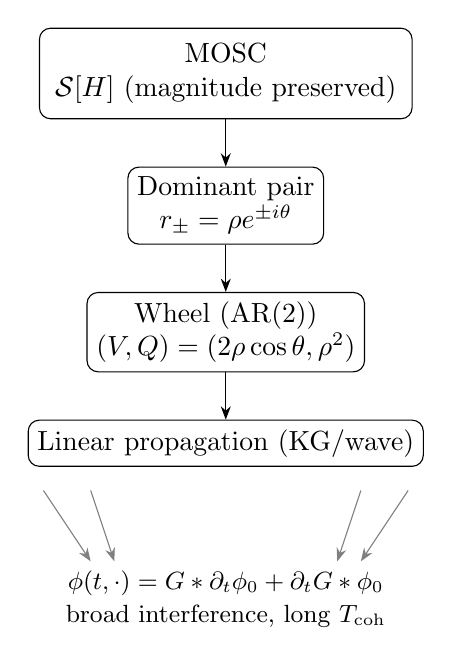
\begin{tikzpicture}[>=Stealth, node distance=6mm]
\node[draw, rounded corners, align=center, inner sep=2mm] (mosc) {MOSC \\ $\mathcal{S}[H]$ (magnitude preserved)};
\node[draw, rounded corners, below=of mosc, align=center] (pair) {Dominant pair \\ $r_\pm=\rho e^{\pm i\theta}$};
\node[draw, rounded corners, below=of pair, align=center] (wheel) {Wheel (AR(2)) \\ $(V,Q)=(2\rho\cos\theta,\rho^2)$};
\node[draw, rounded corners, below=of wheel, align=center, minimum width=4.8cm] (prop) {Linear propagation (KG/wave)};
\draw[->] (mosc) -- (pair);
\draw[->] (pair) -- (wheel);
\draw[->] (wheel) -- (prop);
\coordinate (A) at ($(prop.south west)+(0.2,-0.3)$);
\coordinate (B) at ($(prop.south east)+(-0.2,-0.3)$);
\draw[gray,->] (A) -- ++(0.6,-0.9);
\draw[gray,->] ($(A)+(0.6,0)$) -- ++(0.3,-0.9);
\draw[gray,->] ($(B)+(-0.6,0)$) -- ++(-0.3,-0.9);
\draw[gray,->] (B) -- ++(-0.6,-0.9);
\node[below=12mm of prop, align=center] (sum) {\small $\phi(t,\cdot)=G*\partial_t\phi_0+\partial_tG*\phi_0$ \\ \small broad interference, long $T_{\rm coh}$};
\end{tikzpicture}
\caption{AR(2) coherent superposition}
\end{subfigure}\hfill
\begin{subfigure}[t]{0.48\linewidth}
\centering
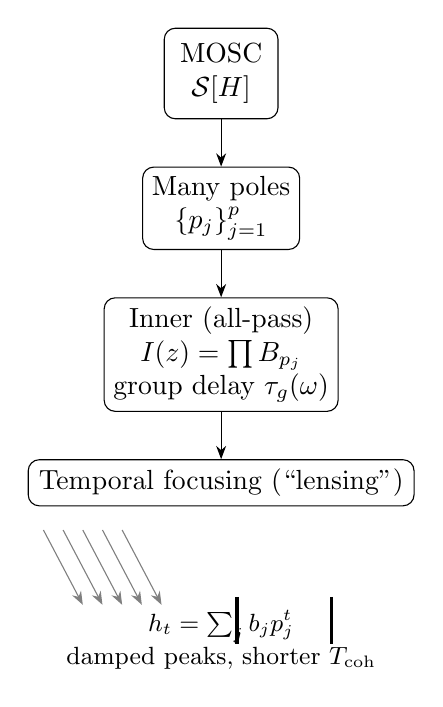
\begin{tikzpicture}[>=Stealth, node distance=6mm]
\node[draw, rounded corners, align=center, inner sep=2mm] (mosc2) {MOSC \\ $\mathcal{S}[H]$};
\node[draw, rounded corners, below=of mosc2, align=center] (many) {Many poles \\ $\{p_j\}_{j=1}^p$};
\node[draw, rounded corners, below=of many, align=center] (inner) {Inner (all-pass) \\ $I(z)=\prod B_{p_j}$ \\ group delay $\tau_g(\omega)$};
\node[draw, rounded corners, below=of inner, align=center, minimum width=4.9cm] (focus) {Temporal focusing (``lensing'')};
\draw[->] (mosc2) -- (many);
\draw[->] (many) -- (inner);
\draw[->] (inner) -- (focus);
\coordinate (L) at ($(focus.south west)+(0.2,-0.3)$);
\foreach \x in {0,0.25,0.5,0.75,1.0} {
  \draw[gray,->] ($(L)+(\x,0)$) -- ++(0.5,-0.95);
}
\draw[very thick] ($(focus.south)+(0.2,-1.15)$) -- ++(0,-0.6);
\draw[very thick] ($(focus.south)+(1.4,-1.15)$) -- ++(0,-0.6);
\node[below=12mm of focus, align=center] {\small $h_t=\sum_j b_j p_j^t$ \\ \small damped peaks, shorter $T_{\rm coh}$};
\end{tikzpicture}
\caption{AR($p$) temporal lensing}
\end{subfigure}
\caption{AR(2) coherent superposition vs.\ AR($p$) temporal lensing.}
\label{fig:superposition-lensing-fig}
\end{figure}

\section{Operational dephasing and coherence decay}
Demodulate by $r_+$, write $z_t=A_t e^{i\phi_t}$, and define $\delta_t=\mathrm{wrap}(\phi_{t+1}-\phi_t)$. Under weak dependence,
\begin{theorem}
If $S_\delta(0)$ exists (Abel-regularized), then $\abs{\mathcal C(t)}\approx \rho^t e^{-Dt}$ with $D=\tfrac12 S_\delta(0)$.
\end{theorem}

\section{Measurement as APBC flips \& the double-slit}
Micro-absorbers indexed by $i$ at $x_i$ carry two states: PBC/APBC with $\sigma_i=\pm1$. A PBC$\to$APBC flip imposes a $\pi$ mark $V\mapsto -V$, $Q$ unchanged; flips inject poles and increase local $S_\delta$ (\emph{topological decoherence}). For small flux, use the hazard
\begin{equation}
\lambda_i^+(t)=\kappa_i\abs{\phi(t,x_i)}^2,\qquad \lambda_i^-\approx0.
\end{equation}
First-arrival yields Born statistics $p(x)\propto \kappa(x)\int\abs{\phi(t,x)}^2 dt$. For a double slit with $\phi=\phi_1+\phi_2$,
\begin{equation}
p(x)\ \propto\ \kappa(x)\,\Big(\abs{\phi_1}^2+\abs{\phi_2}^2+2\abs{\phi_1\phi_2}\cos\Delta\varphi\Big).
\end{equation}
Which-path tagging suppresses the cross term by $\chi\approx e^{-D_{\rm proper}T_{\rm proper}}$; in a stationary detector $D=D_{\rm proper}$, $T=T_{\rm proper}$.

\section{Lorentz invariance: status, conditions, and proof-of-principle}\label{sec:lorentz}
\subsection{Operational definition and status}
We take $\eta=\mathrm{diag}(1,-1,-1,-1)$ and $\Box=\frac{1}{c^2}\partial_t^2-\nabla^2$. The full discrete pipeline is not exactly LI (spatial envelope, telegraph term, coordinate-time dephasing), but the coherent AR(2) core has an LI continuum limit.

\subsection{Sufficient conditions and theorem}
Assume unitary wheel ($Q{=}1$), isotropic local coupling with dispersion $\omega^2(\bm k)=c^2\norm{\bm k}^2+m^2+\bigO(a^2\norm{\bm k}^4)$, and a vanishing/covariant regulator. Then:
\begin{theorem}[AR(2)$\Rightarrow$ KG]
As $a,\tau\to0$ with $a/\tau\to c$, the operator-valued AR(2) update
\(
\phi_{t+\tau}-V(\Delta_a)\phi_t+\phi_{t-\tau}=0
\)
with $V(\Delta_a)=2+\tau^2(c^2\Delta_a-m^2)$ converges to
\(
\frac{1}{c^2}\partial_t^2\phi-\nabla^2\phi+m^2\phi=0,
\)
with truncation error $\mathcal O(\tau^2,a^2)$ in the principal symbol (under the stated regularity).
\end{theorem}

\subsection{Dynamic envelope and effective metric}
Let
\begin{equation}
s(x,t)=s_0+\alpha\,S_\delta(0,x,t),\qquad \sigma=\frac{s}{\tau^2},\qquad c_{\rm eff}^2=c^2-2\sigma.
\end{equation}
Then the wave equation becomes
\begin{equation}
\frac{1}{c^2}\partial_t^2\phi-\frac{c_{\rm eff}^2(x,t)}{c^2}\nabla^2\phi+m^2\phi=0,
\end{equation}
which is the KG equation in an effective metric $g^{00}=1$, $g^{ij}=-(c_{\rm eff}^2/c^2)\delta^{ij}$ up to gradients of $c_{\rm eff}$ (WKB). Null rays follow $g$-geodesics; weak-field identification $\sigma\simeq \gamma_\sigma \Phi$ reproduces Shapiro-like delays and lensing.

\section{Quasi-static gravity and dynamic closure}\label{sec:newton-tele}
Define the operational potential
\begin{equation}
\Phi(x)\defeq \gamma_G\,\tau\,S_\delta(0,x).
\end{equation}
In quasi-static regimes,
\begin{equation}
(\nabla^2-\lambda_s^{-2})\Phi=\tilde\kappa\,S_\delta(0),\qquad \lambda_s\propto \sqrt{s}.
\end{equation}
A dynamic closure respecting the speed bound is
\begin{equation}
\partial_t^2\Phi+2\Gamma\,\partial_t\Phi-c_{\rm eff}^2\nabla^2\Phi+c_{\rm eff}^2\lambda_s^{-2}\Phi=\kappa_d\,\partial_t S_\delta(0,x,t).
\end{equation}

\section{APBC on a ring: a binary probe}
On a ring of length $L$, PBC imposes $y_{n+L}=y_n$, APBC $y_{n+L}=-y_n$.
APBC is equivalent to a Bloch-phase twist of $\Delta\theta=\pi/L$ per site, i.e., $\theta\mapsto\theta+\pi/L$.
For the stride-$L$ decimated law, this induces
$V_L\propto\cos(L\theta+\pi)=-\cos(L\theta)$, hence a \emph{sign flip of $V_L$} while $Q_L$ is unchanged.
This cleanly diagnoses the clock sector.

\section{Estimation pipeline (end-to-end)}\label{sec:pipeline}
\begin{algobox}
\textbf{Inputs:} stream $x_t$, stride $\ell$, (optional) spatial graph, envelope parameterization.\\
\textbf{Outputs:} $(\rho,\theta)$ or $(V,Q)$; $D$; $\Phi$; diagnostics.

\begin{enumerate}[leftmargin=2em,label=\arabic*.]
\item Decimate: $y^{(r)}_k=x_{r+k\ell}$.
\item MOSC-filter and fit AR(2): estimate $(V,Q)$; map to $(\rho,\theta)$ using \eqref{eq:wheel}.
\item Demodulate by $r_+$ and compute wrapped phase increments $\delta_t$.
\item Estimate $S_\delta(0)$ via Abel/radial regularization; set $D=\tfrac12 S_\delta(0)$.
\item If spatial: choose $\mathsf L$; set $s$ (or $s(x)$); infer $\lambda_s$ and $v_{\max}$.
\item Construct $\Phi=\gamma_G\tau S_\delta(0)$; solve screened Poisson (or dynamic closure).
\item Optional APBC probe: verify $V\mapsto -V$, $Q$ unchanged.
\item Report metrics: $\mathcal C_2, N_{\rm eff}, D, T_{\rm coh}$ and residual diagnostics.
\end{enumerate}
\end{algobox}

\section{Diagnostics, units, and failure modes}
\paragraph{Units.} $D$ has $1/\text{time}$; $V,Q$ are dimensionless.
If $\mathsf L$ has units $1/\text{length}$, then $\mathsf L^\dagger\mathsf L$ has $1/\text{length}^2$ and the envelope
$E=\exp(-s\,\mathsf L^\dagger\mathsf L)$ requires $s$ to have units of $\text{length}^2$.
Then $\lambda_s\propto\sqrt{s}$ has units of length, and $\sigma\defeq s/\tau^2$ has units of velocity$^2$,
making $c_{\rm eff}^2=c^2-2\sigma$ dimensionally consistent.

\paragraph{Diagnostics.} Dominant pair validity (AR(2) vs.\ AR($p$)); MOSC stability ($\abs{H}$ invariant); stationarity of $\delta_t$; envelope influence monotonic in $s$; APBC flip check.

\paragraph{Failure modes.} Multiple comparable pairs (need AR($p$)); heavy phase slips; near-unit-circle singularities (regularize radially); graph anisotropy (reweight or continuum Laplace--Beltrami).

\section{Glossary of non-standard terms}
\begin{longtable}{@{}p{0.27\linewidth}p{0.69\linewidth}@{}}
\toprule
Term & Meaning \\ \midrule
\textbf{Residue track} & A decimated subsequence $y_k^{(r)}=x_{r+k\ell}$ for fixed residue $r$ modulo stride $\ell$.\\
\textbf{Reduced transfer} & A $2\times2$ map $M$ that advances a two-dimensional sufficient state across decimated steps; its $\tr,\det$ generate the exact two-step law via Cayley--Hamilton.\\
\textbf{Wheel (AR(2) dictionary)} & $(\rho,\theta)\leftrightarrow(V,Q)$ with $V=2\rho\cos\theta$, $Q=\rho^2$; stride-$\ell$ generalization $V_\ell=2\rho^\ell\cos(\ell\theta)$, $Q_\ell=\rho^{2\ell}$.\\
\textbf{MOSC} & Mirror--Outer Spectral Content: $\mathcal S[H]=H/I$ with $I$ inner; preserves magnitude while removing all-pass phase.\\
\textbf{$\Omega$-compatibility} & Equality of Abel-regularized spectral magnitudes for $H$ and $\mathcal S[H]$.\\
\textbf{APBC} & Anti-periodic boundary condition: $y_{n+L}=-y_n$; induces $\theta\mapsto\theta+\pi/L$ and flips $V_L$ at stride $L$ while $Q_L$ is unchanged.\\
\textbf{Topological decoherence} & Increase in $S_\delta(0)$ and local AR order due to APBC flips (boundary/topological changes), not just additive noise.\\
\textbf{Operational potential} & $\Phi=\gamma_G\tau S_\delta(0)$; in quasi-static limit obeys a screened Poisson equation.\\
\textbf{Dynamic envelope} & $s(x,t)=s_0+\alpha S_\delta(0,x,t)$; renormalizes local speed and defines an effective metric.\\
\bottomrule
\end{longtable}

\appendix

\section{Cayley--Hamilton proof of the decimated two-step law}
Let $u_k\in\C^2$ evolve as $u_{k+1}=M^\ell u_k$. Since $(M^\ell)^2-(\tr M^\ell)M^\ell+(\det M^\ell)\Id=0$, applying both sides to $u_k$ and reading out $y_k=\alpha^\top u_k$ gives \eqref{eq:two-step}.

\section{MOSC factorization details}
For rational $H$, the inner factor is a finite Blaschke product; dividing by it leaves an outer representative with identical boundary magnitude. Equality of Abel-regularized magnitudes follows from radial $L^2$ convergence.

\section{Dephasing decay derivation}
Write $\phi_t=\sum_{j=0}^{t-1}\delta_j+\phi_0$. Then $\mathcal C(t)=\E[e^{i\sum_{j=0}^{t-1}\delta_j}]$. The cumulant expansion and weak dependence give $\log \mathcal C(t)\approx -\tfrac12 \Var(\sum_{j=0}^{t-1}\delta_j)$. Abel-regularizing the triangular covariance sum yields the rate $D=\tfrac12 S_\delta(0)$.

\section{Speed and screening derivation}
Diagonalize in $\mathsf L^\dagger\mathsf L$-eigenmodes. The envelope multiplies mode $\lambda$ by $e^{-s\lambda^2}$; group velocities are suppressed by at most $1/(1+s\lambda^2)$, giving $v_{\max}\lesssim v_0/(1+s\Lambda_{\max}^2)$ and $\lambda_s\propto\sqrt{s}$.

\section{Finite-loop holonomy bound (sketch)}
Compare envelope-updated ordered products with the path-ordered exponential of the Levi--Civita connection via a non-Abelian Stokes estimate; bound the mismatch by curvature variation, discretization, and envelope bias terms.

\section{Green function on a ring}
For net-zero sources on a ring of $L$ sites with AR(2) parameters $(V,Q)$, the Green function is
\begin{equation}
G^{(L)}_n=\frac{1}{L}\sum_{k=0}^{L-1}\frac{e^{2\pi i k n/L}}{V-2\sqrt{Q}\cos(2\pi k/L)},\qquad x=G^{(L)}\!*\,s.
\end{equation}

\section{Ray tracing and Shapiro delay in an $S_\delta$ profile}\label{app:ray}
\subsection{Rays in the effective metric}
With refractive index $n(x)=c/c_{\rm eff}(x)$, Fermat's principle yields
\(
\frac{d}{ds}(n\,\dot{\bm x})=\nabla n(\bm x).
\)
For a weak Gaussian profile $\Phi(\bm x)=\Phi_0 e^{-\norm{\bm x}^2/2R^2}$ and $n\approx 1+\varepsilon e^{-r^2/2R^2}$ with $\varepsilon=\gamma_\sigma \Phi_0/c^2$,
\begin{equation}
\alpha(b)\approx \varepsilon\,\frac{\sqrt{2\pi}\,b}{R}\,e^{-b^2/2R^2},\qquad
\Delta T(b)\approx \frac{\varepsilon\,\sqrt{2\pi}\,R}{c}\,e^{-b^2/2R^2}.
\end{equation}

\subsection{Numerical ray tracer (pseudocode)}
\begin{lstlisting}[style=codeblock,language=Python,caption={RK4 ray tracing in 2D with Gaussian $n(x)$}]
import numpy as np

def n_of_x(x, y, eps=1e-3, R=1.0):
    r2 = x*x + y*y
    return 1.0 + eps*np.exp(-0.5*r2/(R*R))

def grad_n(x, y, eps=1e-3, R=1.0):
    r2 = x*x + y*y
    coeff = -(eps*np.exp(-0.5*r2/(R*R)))/(R*R)
    return coeff*np.array([x, y])  # grad of n-1

def rk4_step(x, v, h, eps=1e-3, R=1.0):
    def accel(x, v):
        g = grad_n(x[0], x[1], eps, R)
        n = n_of_x(x[0], x[1], eps, R)
        vhat = v/np.linalg.norm(v)
        g_perp = g - np.dot(g, vhat)*vhat
        return g_perp / n
    k1x, k1v = v,                accel(x, v)
    k2x, k2v = v + 0.5*h*k1v,    accel(x + 0.5*h*k1x, v + 0.5*h*k1v)
    k3x, k3v = v + 0.5*h*k2v,    accel(x + 0.5*h*k2x, v + 0.5*h*k2v)
    k4x, k4v = v + h*k3v,        accel(x + h*k3x,     v + h*k3v)
    x_next = x + (h/6.0)*(k1x + 2*k2x + 2*k3x + k4x)
    v_next = v + (h/6.0)*(k1v + 2*k2v + 2*k3v + k4v)
    v_next = v_next/np.linalg.norm(v_next)
    return x_next, v_next
\end{lstlisting}

\section*{Acknowledgments}
This master document unifies multiple drafts into a single coherent presentation with expanded explanations of all non-standard terms.
\end{document}
